% !TeX program = xelatex
% !TeX encoding = UTF-8
% !TeX TXS-program:compile = txs:///xelatex | txs:///xelatex
\documentclass[aspectratio=169, table, 12pt]{beamer}
% Preamble bersama seluruh slide mata kuliah ini.
% Dipanggil dari slides/sessionXX/sessionXX.tex tepat sesudah baris
% \documentclass[aspectratio=169, table, 12pt]{beamer}
% Paket tambahan yang hanya dibutuhkan satu sesi ditulis di berkas sesi itu.

\usepackage{colortbl}
\usepackage{xcolor}
\usepackage{listings}
\usepackage{tabularx}
\usepackage{booktabs}
\usepackage{tikz}
\usepackage{pgfplots}
\pgfplotsset{compat=1.18}
\usetikzlibrary{arrows.meta, positioning, calc, fit, shapes.geometric,
	shapes.multipart, backgrounds, matrix, chains, trees}

\makeatletter
\def\input@path{{../theme/}}
\makeatother
\graphicspath{{../theme/}{../../figures/}}
\usetheme{Pradita}

\definecolor{praditagreen}{RGB}{37, 113, 71}

% Tema membuat garis tabel berwarna putih. Dikembalikan agar tabel terbaca.
\arrayrulecolor{black}
\setlength{\arrayrulewidth}{0.5pt}

\lstdefinelanguage{yaml}{
	basicstyle=\ttfamily\scriptsize,
	keywordstyle=\color{blue}\bfseries,
	commentstyle=\color{gray}\itshape,
	stringstyle=\color{red},
	showstringspaces=false,
	breaklines=true,
	frame=lines,
	numbers=none,
	backgroundcolor=\color{lightgray!10},
	tabsize=2,
	morecomment=[l]{\#}
}

\lstdefinelanguage{json}{
	basicstyle=\ttfamily\scriptsize,
	stringstyle=\color{red},
	commentstyle=\color{gray},
	breaklines=true,
	showstringspaces=false,
	tabsize=2,
	numbers=none,
	frame=lines,
	backgroundcolor=\color{lightgray!10},
	string=[s]{"}{"}
}

\lstdefinelanguage{bash}{
	keywords={},
	basicstyle=\ttfamily\scriptsize,
	ndkeywords={docker, kubectl, helm, curl, git, terraform},
	ndkeywordstyle=\color{purple}\bfseries,
	sensitive=true,
	commentstyle=\color{gray},
	numbers=none,
	breaklines=true,
	frame=lines,
	backgroundcolor=\color{lightgray!10},
	tabsize=2,
	comment=[l]{\#},
	showstringspaces=false
}

\lstdefinelanguage{http}{
	keywords={GET, POST, PUT, PATCH, DELETE, HEAD, OPTIONS, HTTP},
	basicstyle=\ttfamily\scriptsize,
	keywordstyle=\color{blue}\bfseries,
	sensitive=true,
	numbers=none,
	breaklines=true,
	frame=lines,
	backgroundcolor=\color{lightgray!10},
	tabsize=2,
	showstringspaces=false
}

\subtitle{IT40613 · Digital Platform \& API Economy}
\author{\textbf{Alfa Yohannis}}


\title{\Huge Developer Experience\\ \vspace{10pt} dan Portal Pengembang}
\date{Pertemuan 11}

\begin{document}
\frame{\titlepage}

\begin{frame}
  \frametitle{Isi Pertemuan}
  \vspace{14pt}
  \begin{columns}[t]
    \column{0.5\textwidth}
    {\small\tableofcontents[sections={1-5}]}

    \column{0.5\textwidth}
    {\small\tableofcontents[sections={6-10}]}
  \end{columns}
\end{frame}

\begin{frame}{\hfill}
  \centering
  \Huge{\textbf{Membaca panduan: 20 menit.\\Menunggu akun uji: 2 hari kerja.\\Dokumen mana yang salah?}}
\end{frame}

\section{Tujuan dan Konteks}

\begin{frame}{{\Large Tujuan Pembelajaran}}
  \vspace{10pt}
  \begin{itemize}
    \item Menjelaskan unsur \textit{developer experience} yang menentukan cepat atau lambatnya mitra terhubung.
    \item Merancang alur \textit{onboarding} mitra dari pendaftaran sampai produksi.
    \item Menyusun kerangka portal pengembang beserta ukuran keberhasilannya.
  \end{itemize}
\end{frame}

\begin{frame}{{\Large Diagram Konsep Bab 11}}
  \centering
  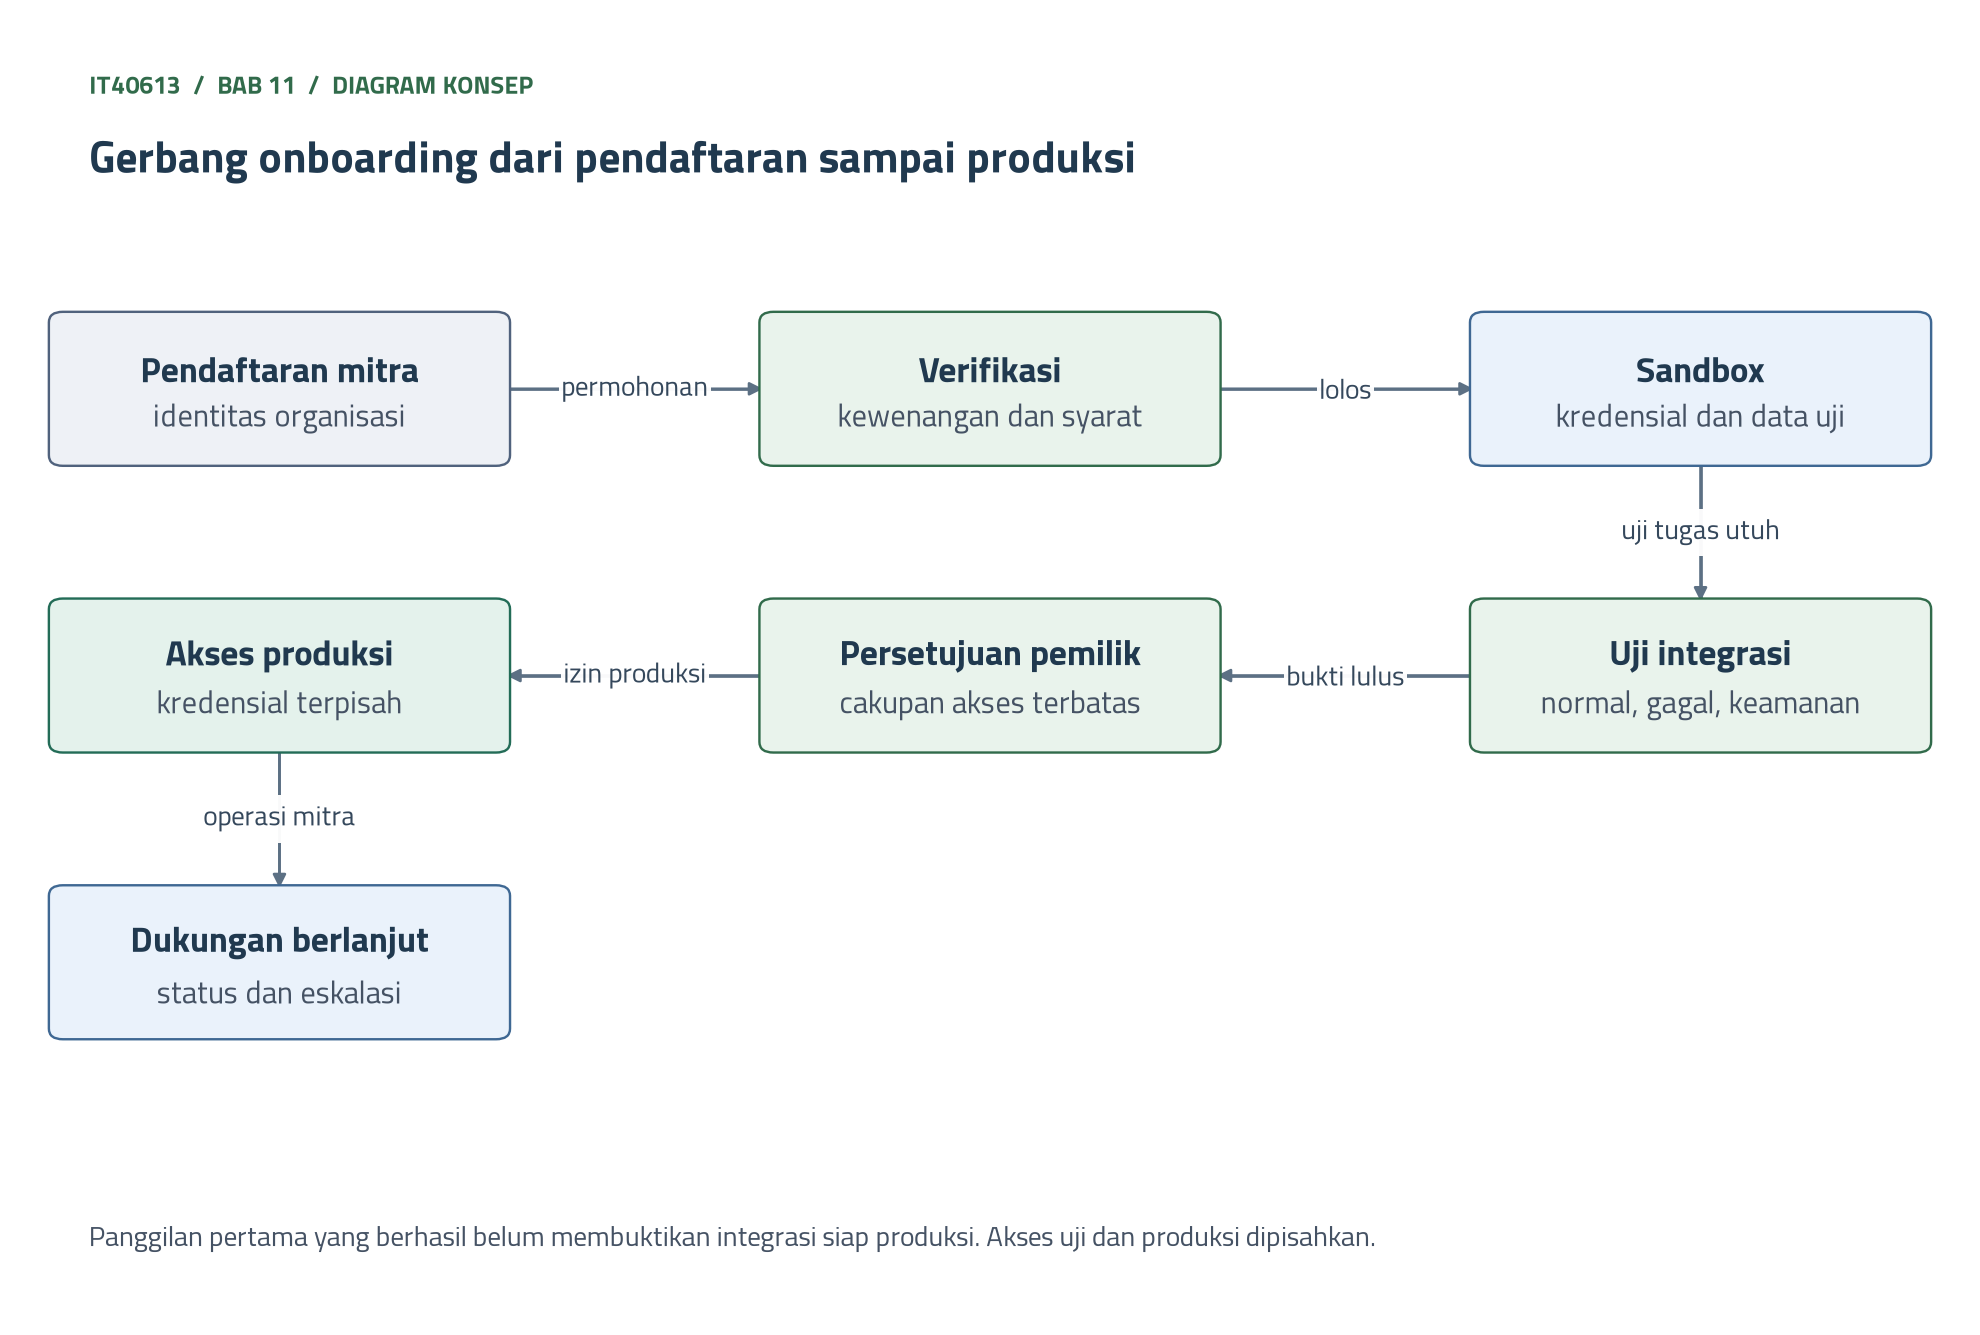
\includegraphics[width=0.96\textwidth,height=0.77\textheight,keepaspectratio]{../../figures/ch11-diagram-konsep.png}
\end{frame}

\begin{frame}{{\Large Masukan dari Bab Sebelumnya}}
  \footnotesize
  \begin{tabularx}{\textwidth}{>{\raggedright\arraybackslash}p{1.3cm} >{\raggedright\arraybackslash}X >{\raggedright\arraybackslash}p{4.6cm}}
    \hline
    \textbf{Asal} & \textbf{Temuan yang dipakai} & \textbf{Kegunaan di sini} \\ \hline
    Bab 3 & Tangga keterbukaan, 20 pasien sintetis, 6 skenario gagal, kuota uji 100 & Gerbang dan \textit{sandbox} \\ \hline
    Bab 5 & Rantai pemesanan 99,40 persen, 168 gagal per bulan & Janji layanan \\ \hline
    Bab 7 & Spesifikasi terdokumentasi dan tersedia & Isi portal \\ \hline
    Bab 9 & Kontrak API-01, 9 tipe masalah & Sumber dokumentasi \\ \hline
    Bab 10 & Alternatif A, ruang Rp30,4 juta per tahun, cadangan 120 jam, transisi 6 bulan & Batas lingkup portal \\ \hline
  \end{tabularx}

  \vspace{8pt}
  \small Tetap dipakai: 40 klinik mitra, kuota 300 per hari per klinik, tarif Rp60.000 per jam, lapisan bersama Rp300 juta per tahun.
\end{frame}

\section{Mitra sebagai Pengguna API}

\begin{frame}{{\Large Siapa Pengguna API?}}
  \vspace{8pt}
  \begin{itemize}
    \item Orang atau tim yang mengerjakan tugas tertentu melalui sistemnya.
    \item Pengguna teknis memerlukan petunjuk implementasi.
    \item Pemilik layanan memerlukan kejelasan proses dan dukungan.
    \item Kebutuhan dipelajari melalui wawancara serta pengamatan.
    \item Persona harus berisi tugas, hambatan, dan konteks keputusan.
  \end{itemize}
  \vspace{6pt}
  {\small Analogi: loket dinilai dari urusan warga yang selesai, bukan banyaknya formulir.}
\end{frame}

\begin{frame}{{\Large Dua Contoh Berangka}}
  \vspace{8pt}
  \begin{itemize}
    \item Satu klinik: 60 pemesanan per hari, 1.500 per bulan, 15 konflik slot.
    \item 40 klinik: 600 konflik per bulan. Bila 409 dibaca sebagai gangguan umum: 30 jam per bulan, Rp21,6 juta per tahun.
    \item Pemilik kemitraan menanyakan status: 40 klinik, 2 kali per minggu, 4 minggu, 15 menit.
    \item Bebannya 80 jam, atau Rp4,8 juta. Dua per tiga dari cadangan 120 jam.
    \item Satu halaman status menghapus sebagian besar pertanyaan itu.
  \end{itemize}
\end{frame}

\begin{frame}{{\Large Yang Sering Tertukar: Klinik dan Pengembang Klinik}}
  \footnotesize
  \begin{tabularx}{\textwidth}{>{\raggedright\arraybackslash}p{2.9cm} >{\raggedright\arraybackslash}X >{\raggedright\arraybackslash}X}
    \hline
    \textbf{Pengguna} & \textbf{Tugas yang ingin selesai} & \textbf{Hambatan} \\ \hline
    Vendor sistem klinik & Memasang API-01 sekali untuk banyak klinik & Perubahan kontrak mengenai banyak klinik \\ \hline
    Teknisi klinik & Membuat janji sah pertama & Akun uji tertunda, arti 409 dan 503 \\ \hline
    Pemilik kemitraan & Menambah klinik aktif & Status persetujuan tidak terlihat \\ \hline
    Petugas pelindungan data & Memastikan data minimum & Data nyata dipakai untuk uji \\ \hline
  \end{tabularx}

  \vspace{8pt}
  \small Misalkan 28 klinik memakai 3 vendor, dan 12 klinik punya teknisi sendiri. Keduanya gagal pada tempat yang berbeda.
\end{frame}

\section{Developer Experience dan Panggilan Pertama}

\begin{frame}{{\Large Developer Experience}}
  \vspace{8pt}
  \begin{itemize}
    \item Mencakup penemuan API, pemahaman kontrak, akses uji, implementasi, pemecahan galat, dan operasi.
    \item Fagerholm dan Münch: cara menangkap bagaimana pengembang berpikir dan merasakan kegiatannya.
    \item \textit{Time to first call}: waktu menuju panggilan awal yang berhasil.
    \item Definisi awal dan akhir harus eksplisit.
    \item Panggilan pertama belum membuktikan integrasi siap produksi.
  \end{itemize}
  \vspace{6pt}
  {\small Analogi: mudah menemukan alamat restoran belum membuktikan makanan diterima sesuai pesanan.}
\end{frame}

\begin{frame}{{\Large Lima Garis Akhir}}
  \centering
  \eadiagram{../../figures/ch11-lapisan-ukuran.tex}
\end{frame}

\begin{frame}{{\Large Yang Sering Tertukar: Waktu Kerja dan Waktu Tunggu}}
  \centering
  \eadiagram{../../figures/ch11-perjalanan-mitra.tex}
\end{frame}

\begin{frame}{{\Large Membaca Perjalanan Satu Klinik}}
  \vspace{8pt}
  \begin{itemize}
    \item Saat ini 156,5 jam, atau 19,6 hari kerja. 128 jam, atau 82 persen, adalah tunggu.
    \item Panggilan pertama pada jam ke-42,5, padahal kerja klinik hanya 2,5 jam.
    \item Sasaran: 6,5 jam untuk panggilan pertama, 7,6 hari kerja untuk seluruh tahap.
    \item Hemat 12 hari kerja: Rp1,44 juta per klinik, Rp57,6 juta untuk 40 klinik, sekali saja.
    \item Sumber yang ditelaah tidak memberi angka baku. Sasaran dihitung dari perjalanan sendiri.
  \end{itemize}
\end{frame}

\begin{frame}{{\Large Hasil Lima Klinik Uji}}
  \footnotesize
  \begin{tabularx}{\textwidth}{>{\raggedright\arraybackslash}p{1.1cm} >{\raggedright\arraybackslash}p{2.6cm} >{\raggedright\arraybackslash}p{1.8cm} >{\raggedright\arraybackslash}p{1.35cm} >{\raggedright\arraybackslash}p{1.55cm} >{\raggedright\arraybackslash}X}
    \hline
    \textbf{Klinik} & \textbf{Kelompok} & \textbf{Panggilan pertama} & \textbf{Tugas normal} & \textbf{Skenario gagal} & \textbf{Berhenti terlama} \\ \hline
    U1 & Vendor A & 20 menit & 3 dari 3 & 5 dari 6 & Membaca 503 \\ \hline
    U2 & Vendor A & 25 menit & 3 dari 3 & 5 dari 6 & Membaca 503 \\ \hline
    U3 & Vendor B & 30 menit & 3 dari 3 & 4 dari 6 & Membaca 429 \\ \hline
    U4 & Teknisi sendiri & 40 menit & 2 dari 3 & 3 dari 6 & Kunci idempotensi \\ \hline
    U5 & Teknisi sendiri & 150 menit & 1 dari 3 & 2 dari 6 & Memperoleh token \\ \hline
  \end{tabularx}

  \vspace{6pt}
  \small Median 30, rata-rata 53 menit. Tugas normal 12 dari 15. Skenario gagal 19 dari 30. Seluruh angka adalah pemisalan.
\end{frame}

\begin{frame}{{\Large Kasus Medikara: Lima Klinik Uji}}
  \vspace{4pt}
  \begin{itemize}
    \item U5 tidak dibuang, karena mewakili kelompok 12 klinik.
    \item U1 dan U2 memakai vendor sama, sehingga temuan 503 baru satu pengamatan.
    \item Nielsen: 5 peserta sekitar 85 persen masalah, bila $L$ 31 persen dan pengguna sebanding.
    \item Dua kelompok: 3 sampai 4 peserta per kelompok. U6 ditambahkan.
    \item Keputusan: perbaiki proses dulu, lalu panduan galat untuk 6 skenario.
  \end{itemize}
\end{frame}

\section{Dokumentasi, Sandbox, dan SDK}

\begin{frame}{{\Large Referensi, Panduan, dan Contoh}}
  \vspace{4pt}
  \footnotesize
  \begin{tabularx}{\textwidth}{>{\raggedright\arraybackslash}p{2.2cm} >{\raggedright\arraybackslash}p{3.4cm} >{\raggedright\arraybackslash}X >{\raggedright\arraybackslash}p{2.9cm}}
    \hline
    \textbf{Bentuk} & \textbf{Kebutuhan} & \textbf{Isi pada API-01} & \textbf{Dipelihara} \\ \hline
    Tutorial & Belajar sambil melakukan & Panduan mulai cepat & Diuji rekan baru \\ \hline
    \textit{How-to guide} & Menyelesaikan satu tugas & Menangani 409, pindah ke \texttt{/v2} & Dari tiket berulang \\ \hline
    \textit{Reference} & Mencari rincian & 4 operasi, 9 tipe masalah & Dari kontrak \\ \hline
    \textit{Explanation} & Memahami alasan & Arti terkonfirmasi, tingkat akses & Pemilik produk \\ \hline
  \end{tabularx}

  \vspace{6pt}
  \small Diátaxis: tindakan atau pemahaman, memperoleh atau menerapkan keterampilan. Contoh hadir di keempatnya.
\end{frame}

\begin{frame}{{\Large Mengapa Lengkap Belum Cukup?}}
  \vspace{8pt}
  \begin{itemize}
    \item Uddin dan Robillard, 323 pengembang: terberat ambiguitas, tidak lengkap, dan salah isi.
    \item Enam dari sepuluh masalah memaksa pengembang beralih ke API lain.
    \item Robillard: pengembang tetap perlu cara menemukan informasi.
    \item Postman 2025: 55 persen dokumentasi tidak konsisten, 34 persen API tidak ditemukan.
    \item Angka Postman menggambarkan kolaborasi tim API, bukan khusus mitra.
  \end{itemize}
\end{frame}

\begin{frame}{{\Large Dua Contoh Berangka: Dokumentasi}}
  \vspace{8pt}
  \begin{itemize}
    \item Panduan awal memangkas pendampingan dari 24 jam ke 4 jam per klinik.
    \item 40 klinik: Rp57,6 juta menjadi Rp9,6 juta pada tarif Rp60.000 per jam, sama dengan Bab 3.
    \item 24 perubahan per tahun, 3 tempat disunting: 72 jam per tahun.
    \item Referensi dibangkitkan dari kontrak: tinggal 48 jam.
  \end{itemize}
  \vspace{6pt}
  {\small Analogi: buku manual, resep, dan contoh masakan mempunyai fungsi yang berbeda.}
\end{frame}

\begin{frame}{{\Large Sandbox dan Data Uji Sintetis}}
  \vspace{8pt}
  \begin{itemize}
    \item Lingkungan aman yang meniru produksi dengan jawaban simulasi.
    \item Regulasi 2018/389 Pasal 30 ayat 5: fasilitas uji, tanpa informasi sensitif.
    \item Epic: untuk pengujian, hanya data sampel atau sintetis.
    \item Stripe: nomor kartu uji yang pasti berhasil dan pasti ditolak.
    \item \textit{Sandbox} tidak menggantikan uji pada 5 SIMRS.
  \end{itemize}
  \vspace{6pt}
  {\small Analogi: manekin di ruang latihan perawat. Kesalahan tidak mencederai siapa pun.}
\end{frame}

\begin{frame}{{\Large Enam Skenario Gagal API-01}}
  \footnotesize
  \begin{tabularx}{\textwidth}{>{\raggedright\arraybackslash}p{3.0cm} >{\raggedright\arraybackslash}p{4.9cm} >{\raggedright\arraybackslash}X}
    \hline
    \textbf{Skenario} & \textbf{Kode dan tipe masalah} & \textbf{Perilaku klinik} \\ \hline
    Pasien tidak ditemukan & 400 \texttt{pasien-tidak-dapat-dipakai} & Periksa nomor \\ \hline
    Slot penuh & 409 \texttt{slot-terisi} & Tawarkan slot lain \\ \hline
    Kode akses kedaluwarsa & 401 \texttt{token-tidak-sah} & Minta token baru \\ \hline
    Kuota habis & 429 \texttt{kuota-habis} & Tunda sesuai \texttt{Retry-After} \\ \hline
    Format salah & 400 \texttt{masukan-tidak-sah} & Perbaiki isian \\ \hline
    SIMRS diperbarui & 503 \texttt{simrs-tidak-tersedia} & Coba lagi \\ \hline
  \end{tabularx}

  \vspace{6pt}
  \small Penjamin menolak berada di luar API-01, sesuai Bab 9. Kuota uji 100 panggilan per hari.
\end{frame}

\begin{frame}{{\Large SDK dan Koleksi Contoh Permintaan}}
  \vspace{8pt}
  \begin{itemize}
    \item \textit{Software Development Kit} (SDK) membungkus panggilan API dalam satu bahasa.
    \item Misalkan 4 bahasa: 480 jam, Rp28,8 juta, ditambah 160 jam per tahun.
    \item Koleksi contoh: 24 jam per tahun. Cadangan hanya 120 jam.
    \item Lin: 17 menit menjadi 10 menit dengan koleksi. Sumbernya vendor, metode tidak dirinci.
    \item SDK terlambat 2 bulan: klinik tinggal 4 dari 6 bulan masa transisi.
  \end{itemize}
  \vspace{6pt}
  {\small Analogi: contoh formulir murah. Biro jasa harus dibayar dan tahu setiap perubahan aturan.}
\end{frame}

\section{Portal dan Katalog API}

\begin{frame}{{\Large Portal Pengembang dan Katalog API}}
  \vspace{8pt}
  \begin{itemize}
    \item Portal: katalog, dokumentasi, pendaftaran, akses, status, dan dukungan.
    \item Katalog: pemilik, audiens, versi, serta status siklus hidup.
    \item Kerangka informasi mengikuti pertanyaan pengguna.
    \item Bukan kewajiban membeli produk baru. Kebutuhan dipenuhi bertahap.
    \item Status layanan menghemat 87,5 jam, atau Rp5,25 juta per tahun, pada pembaruan SIMRS.
  \end{itemize}
  \vspace{6pt}
  {\small Analogi: papan informasi dan petugas layanan harus memberi jawaban yang sama.}
\end{frame}

\begin{frame}{{\Large Kerangka Portal}}
  \centering
  \eadiagram{../../figures/ch11-peta-portal.tex}
\end{frame}

\begin{frame}{{\Large Empat Pilihan Lingkup Portal}}
  \scriptsize
  \begin{tabularx}{\textwidth}{>{\raggedright\arraybackslash}X >{\raggedright\arraybackslash}p{1.9cm} >{\raggedright\arraybackslash}p{1.9cm} >{\raggedright\arraybackslash}p{1.9cm} >{\raggedright\arraybackslash}p{1.9cm}}
    \hline
    \textbf{Juta rupiah, 3 tahun} & \textbf{Tanpa portal} & \textbf{P1 statis} & \textbf{P2 bawaan} & \textbf{P3 kustom} \\ \hline
    Penyiapan & 0 & 14,4 & 24 & 150 \\ \hline
    Pendampingan 40 klinik & 57,6 & 19,2 & 9,6 & 9,6 \\ \hline
    Tiket per tahun & 57,6 & 28,8 & 14,4 & 7,2 \\ \hline
    Isi per tahun & 0 & 2,4 & 3,6 & 18 \\ \hline
    \textbf{Total} & \textbf{230,4} & \textbf{127,2} & \textbf{87,6} & \textbf{235,2} \\ \hline
    Terhadap ruang Rp91,2 juta & 139,2 di atas & 36 di atas & 3,6 di bawah & 144 di atas \\ \hline
    Cadangan 120 jam per tahun & Sisa 120 & Sisa 80 & Sisa 60 & Kurang 180 \\ \hline
    Panggilan pertama & 42,5 jam & 22,5 jam & 6,5 jam & 6,5 jam \\ \hline
  \end{tabularx}

  \vspace{4pt}
  \footnotesize Seluruh angka adalah pemisalan latihan, bukan harga produk.
\end{frame}

\begin{frame}{{\Large Kasus Medikara: Portal dalam Rp91,2 Juta}}
  \vspace{4pt}
  \begin{itemize}
    \item P2 muat hanya bila tiket paling banyak 1,08 per klinik per bulan.
    \item Bila tiket 2: P2 Rp130,8 juta, lebih mahal daripada P1 Rp127,2 juta.
    \item Tahun 1: Rp337,2 juta, di atas pagu Rp37,2 juta. Tahun 2 dan 3: Rp279,6 juta.
    \item Tiga tahun: Rp896,4 juta dari Rp900 juta. Uji coba Rp9,6 juta belum masuk.
    \item Keputusan: P2 bersyarat, tiket diukur 3 bulan. P3 ditolak dengan pemicu tinjauan.
  \end{itemize}
\end{frame}

\begin{frame}{{\Large Ukuran Keberhasilan Portal}}
  \footnotesize
  \begin{tabularx}{\textwidth}{>{\raggedright\arraybackslash}p{4.4cm} >{\raggedright\arraybackslash}p{2.6cm} >{\raggedright\arraybackslash}X}
    \hline
    \textbf{Ukuran} & \textbf{Sasaran} & \textbf{Menyesatkan bila} \\ \hline
    Waktu sampai panggilan pertama & 6,5 jam & Akun dibuatkan sebelum jam mulai \\ \hline
    Tugas selesai tanpa bantuan & 5 dari 6 skenario & Skenario sulit dihapus \\ \hline
    Waktu sampai produksi & 7,6 hari kerja & Syarat dikendurkan \\ \hline
    Tiket per klinik per bulan & 1 tiket & Telepon tidak dihitung \\ \hline
    Aktivasi mitra & Minimal 30 klinik & Pesanan uji di produksi \\ \hline
  \end{tabularx}

  \vspace{6pt}
  \small 4.000 kunjungan per bulan belum bermakna. Analogi: ruang tunggu ramai tidak berarti banyak pasien sembuh.
\end{frame}

\section{Alur Onboarding}

\begin{frame}{{\Large Alur Onboarding dan Verifikasi Mitra}}
  \vspace{8pt}
  \begin{itemize}
    \item Tujuh tahap, sesuai diagram konsep. Lima di antaranya langkah inti.
    \item Persetujuan pemilik: gerbang sebelum akses produksi.
    \item Dukungan berlanjut: keadaan sesudah akses terbit.
    \item Setiap perpindahan punya pemilik, bukti, dan sasaran waktu.
    \item Penghentian mitra dirancang sebelum akses diberikan.
  \end{itemize}
  \vspace{6pt}
  {\small Analogi: kartu pegawai magang tidak membuka ruang arsip.}
\end{frame}

\begin{frame}{{\Large Lingkungan Uji dan Lingkungan Produksi}}
  \centering
  \eadiagram{../../figures/ch11-gerbang-kredensial.tex}
\end{frame}

\begin{frame}{{\Large Bukti dan Pemilik Tiap Tahap}}
  \scriptsize
  \begin{tabularx}{\textwidth}{>{\raggedright\arraybackslash}p{2.7cm} >{\raggedright\arraybackslash}X >{\raggedright\arraybackslash}p{3.1cm} >{\raggedright\arraybackslash}p{1.7cm}}
    \hline
    \textbf{Tahap} & \textbf{Bukti kelulusan} & \textbf{Pemilik} & \textbf{Tunggu} \\ \hline
    Pendaftaran mitra & Identitas organisasi, kontak teknis & Klinik & Tanpa \\ \hline
    Verifikasi & Kewenangan, syarat penggunaan disetujui & Pemilik kemitraan & 4 jam \\ \hline
    \textit{Sandbox} & Kredensial uji, 200 pada jadwal & Sistem portal & Tanpa \\ \hline
    Uji integrasi & 3 tugas, 6 skenario gagal, otorisasi objek & Tim integrasi & 16 jam \\ \hline
    Persetujuan pemilik & Izin usaha, perjanjian, cakupan terbatas & Manajer Rawat Jalan & 16 jam \\ \hline
    Akses produksi & Kredensial terpisah, kuota 300 & Tim integrasi & 4 jam \\ \hline
    Dukungan berlanjut & Kanal, prioritas, status, jadwal tinjau & Layanan pelanggan & Prioritas \\ \hline
  \end{tabularx}
\end{frame}

\begin{frame}{{\Large Yang Sering Tertukar: Verifikasi dan Persetujuan}}
  \vspace{8pt}
  \begin{itemize}
    \item Verifikasi: siapa pemohon, dan apakah ia berwenang. Membuka \textit{sandbox}, tingkat 1 Bab 3.
    \item Persetujuan pemilik: apa yang boleh dilakukan terhadap pasien nyata, tingkat 2 Bab 3.
    \item Izin usaha sebelum \textit{sandbox}: klinik menunggu 24 jam untuk data sintetis.
    \item Laboratorium memerlukan tingkat 3: hubungan layanan aktif, tinjauan 90 hari.
    \item Buka menurut tindakan, bukan menurut pihak.
  \end{itemize}
\end{frame}

\begin{frame}{{\Large Dua Konsekuensi dan Penghentian Mitra}}
  \vspace{8pt}
  \begin{itemize}
    \item Biaya gerbang: 3 orang, 1 jam, Rp180.000 per klinik, Rp7,2 juta untuk 40 klinik.
    \item Satu insiden kecil Rp23,7 juta, sekitar 3,3 kali seluruh biaya gerbang.
    \item Antrean: 10 klinik per minggu, 35 klinik selesai dalam 4 minggu bila bergelombang.
    \item Keluar: identitas klien dicabut, token mati paling lama 15 menit kemudian.
    \item Janji aktif: 300 janji, 3 menit per janji, 15 jam, Rp900.000.
  \end{itemize}
\end{frame}

\section{Syarat, SLA, dan Dukungan}

\begin{frame}{{\Large Syarat Penggunaan dan Tingkat Layanan}}
  \vspace{8pt}
  \begin{itemize}
    \item Syarat penggunaan: tujuan, kewenangan, batas konsumsi, tanggung jawab mitra.
    \item \textit{Service Level Indicator} (SLI): ukuran kuantitatif yang didefinisikan dengan cermat.
    \item \textit{Service Level Objective} (SLO): nilai target yang diukur dengan SLI.
    \item \textit{Service Level Agreement} (SLA): kontrak dengan akibat bila target meleset.
    \item Tanpa akibat tertulis, itu kemungkinan besar SLO.
  \end{itemize}
  \vspace{6pt}
  {\small Analogi: perjanjian sewa menjelaskan cara menangani kerusakan, bukan hanya menyerahkan kunci.}
\end{frame}

\begin{frame}{{\Large Tiga Dokumen, Satu Angka}}
  \footnotesize
  \begin{tabularx}{\textwidth}{>{\raggedright\arraybackslash}p{2.8cm} >{\raggedright\arraybackslash}X >{\raggedright\arraybackslash}p{3.9cm}}
    \hline
    \textbf{Butir} & \textbf{Isi pada contoh} & \textbf{Tempat} \\ \hline
    Kewenangan & Kredensial tidak boleh dibagi & Syarat penggunaan \\ \hline
    Batas konsumsi & Kuota uji 100, produksi 300 & Syarat, perjanjian, kontrak \\ \hline
    Data \textit{sandbox} & Hanya 20 pasien sintetis & Syarat penggunaan \\ \hline
    Tanggung jawab & Hanya 201 berarti terkonfirmasi & Kontrak API, syarat \\ \hline
    Biaya & Rp3 juta per klinik per bulan, usulan & Perjanjian kerja sama \\ \hline
    Perubahan versi & Transisi 6 bulan, tanggal \textit{sunset} & Perjanjian, portal \\ \hline
  \end{tabularx}
\end{frame}

\begin{frame}{{\Large Janji yang Dapat Ditepati}}
  \footnotesize
  \begin{tabularx}{\textwidth}{>{\raggedright\arraybackslash}X >{\raggedright\arraybackslash}p{2.3cm} >{\raggedright\arraybackslash}p{2.3cm} >{\raggedright\arraybackslash}p{2.3cm}}
    \hline
    \textbf{Unsur} & \textbf{SLA 99,9} & \textbf{SLA 99,4} & \textbf{SLA 99,0} \\ \hline
    Gangguan per bulan & 43 menit & 4,32 jam & 7,2 jam \\ \hline
    Bulan meleset per tahun & 12 bulan & 5 bulan & 1 bulan \\ \hline
    Kredit per tahun & Rp144 juta & Rp60 juta & Rp12 juta \\ \hline
    Terhadap Rp1,44 miliar & 10 persen & 4,2 persen & 0,8 persen \\ \hline
  \end{tabularx}

  \vspace{8pt}
  \small Rantai pemesanan 99,40 persen. Kredit 10 persen: Rp300.000 per klinik, Rp12 juta bila seluruh klinik terdampak.
\end{frame}

\begin{frame}{{\Large Kasus Medikara: Janji 99,9 Persen}}
  \vspace{4pt}
  \begin{itemize}
    \item Rata-rata 99,40 persen, sehingga janji 99,9 persen meleset setiap bulan.
    \item Pembaruan SIMRS 7 sampai 14 hari per tahun: 96,2 sampai 98,1 persen bila dihitung.
    \item SLI: pemesanan tanpa 5xx. Pemeliharaan yang diumumkan 14 hari sebelumnya dikecualikan.
    \item SLA 99,0 persen, SLO internal 99,4 persen, selisih 2,88 jam per bulan.
    \item Ditinjau sesudah 3 bulan data nyata. Janji mudah dinaikkan, sulit diturunkan.
  \end{itemize}
\end{frame}

\begin{frame}{{\Large Dukungan dan Komunitas Pengembang}}
  \footnotesize
  \begin{tabularx}{\textwidth}{>{\raggedright\arraybackslash}p{2.0cm} >{\raggedright\arraybackslash}X >{\raggedright\arraybackslash}p{2.2cm} >{\raggedright\arraybackslash}p{3.9cm}}
    \hline
    \textbf{Prioritas} & \textbf{Contoh} & \textbf{Tanggap} & \textbf{Eskalasi} \\ \hline
    1 Kritis & Salah pasien, dugaan kebocoran & 15 menit & Keamanan, pelindungan data \\ \hline
    2 Tinggi & Satu klinik tidak dapat memesan & 1 jam & Tim integrasi \\ \hline
    3 Sedang & Galat tidak jelas, kuota & 4 jam kerja & Tim integrasi \\ \hline
    4 Rendah & Permintaan contoh dokumentasi & 5 hari kerja & Pemilik produk \\ \hline
  \end{tabularx}

  \vspace{6pt}
  \small UU 27/2022 Pasal 46: pemberitahuan paling lambat 3 $\times$ 24 jam. Forum tertutup untuk 41 konsumen, 24 jam moderasi per tahun, bukan jalur laporan insiden.
\end{frame}

\begin{frame}{{\Large Enam Keputusan Bab Ini}}
  \centering
  \eadiagram{../../figures/ch11-peta-keputusan.tex}
\end{frame}

\section{Aktivitas}

\begin{frame}{{\Large Aktivitas: Portal dan Onboarding Mitra}}
  \vspace{4pt}
  \begin{itemize}
    \item Tujuan: alur \textit{onboarding} mitra dan kerangka portal sebagai artefak C3.
    \item Anggota bisnis dan hukum: syarat penggunaan, tingkat layanan, alur persetujuan.
    \item Anggota teknis: kerangka portal dan isi dokumentasi minimum.
    \item Tim: target waktu sampai panggilan pertama, uji panduan dengan rekan baru.
    \item Kaitan: tonggak C3 Kondisi Target. Kriteria: 25, 30, 30, dan 15 persen.
  \end{itemize}
  \vspace{4pt}
  {\footnotesize Berkas pendukung: \berkas{sources/chapter11/README.md}. Pakai data sintetis, atau data berizin yang dianonimkan.}
\end{frame}

\section{Ringkasan}

\begin{frame}{{\Large Ringkasan}}
  \vspace{4pt}
  \begin{itemize}
    \item Mitra terdiri dari orang dengan tugas berbeda, dan sebagian kebutuhannya bukan dokumentasi.
    \item Pisahkan waktu kerja dari waktu tunggu: 82 persen dari 156,5 jam adalah tunggu.
    \item Sarana dipilih menurut kebutuhan pembaca dan kemampuan memeliharanya.
    \item Portal dihitung 3 tahun: P2 Rp87,6 juta muat bila tiket sekitar 1 per klinik per bulan.
    \item Gerbang memisahkan uji dan produksi. Janji dihitung dari rantai, bukan dari harapan.
  \end{itemize}
\end{frame}

\section{Latihan}

\begin{frame}{{\Large Latihan}}
  \vspace{8pt}
  \begin{enumerate}
    \item Jelaskan mengapa dokumentasi yang lengkap belum tentu menghasilkan \textit{developer experience} yang baik.
    \item Susun lima langkah \textit{onboarding} untuk laboratorium mitra, lalu tandai langkah yang paling mungkin menjadi hambatan.
    \item Tentukan tiga ukuran keberhasilan portal pengembang dan jelaskan cara mengumpulkan datanya.
  \end{enumerate}
  \vspace{8pt}
  {\small Setiap latihan punya tabel contoh dan lembar isian pada Bab 11.}
\end{frame}

\end{document}
